\documentclass{beamer}
\usepackage{amsmath}
\usepackage{pgf}
\usepgflibrary{fpu}
\usepackage{pgfplots}
\usepackage{tikz}
\usetikzlibrary{angles,fit,arrows,calc,math,intersections,through,backgrounds}
\usepackage{tkz-euclide}
\usepackage{tkz-graph}
\usepackage{graphicx}

\usetheme{Pittsburgh}
\usecolortheme{seahorse}

\title{Arithmetic expression geometry \\ with an application on learnable non-linearity}
\author[Author] {Mingli Yuan}

\begin{document}
\pgfplotsset{compat=1.18}

\begin{frame}
\maketitle
\end{frame}

\begin{frame}
\frametitle{Table of Contents}
\tableofcontents
\end{frame}

\section{Arithmetic expression geometry: the first glimpse}\label{sec:arithmetic-expression-geometry:first-glimpse}

\begin{frame}
\frametitle{Arithmetic expression geometry: the first glimpse}
\begin{figure}[ht]\centering
\resizebox{0.5\textwidth}{!}{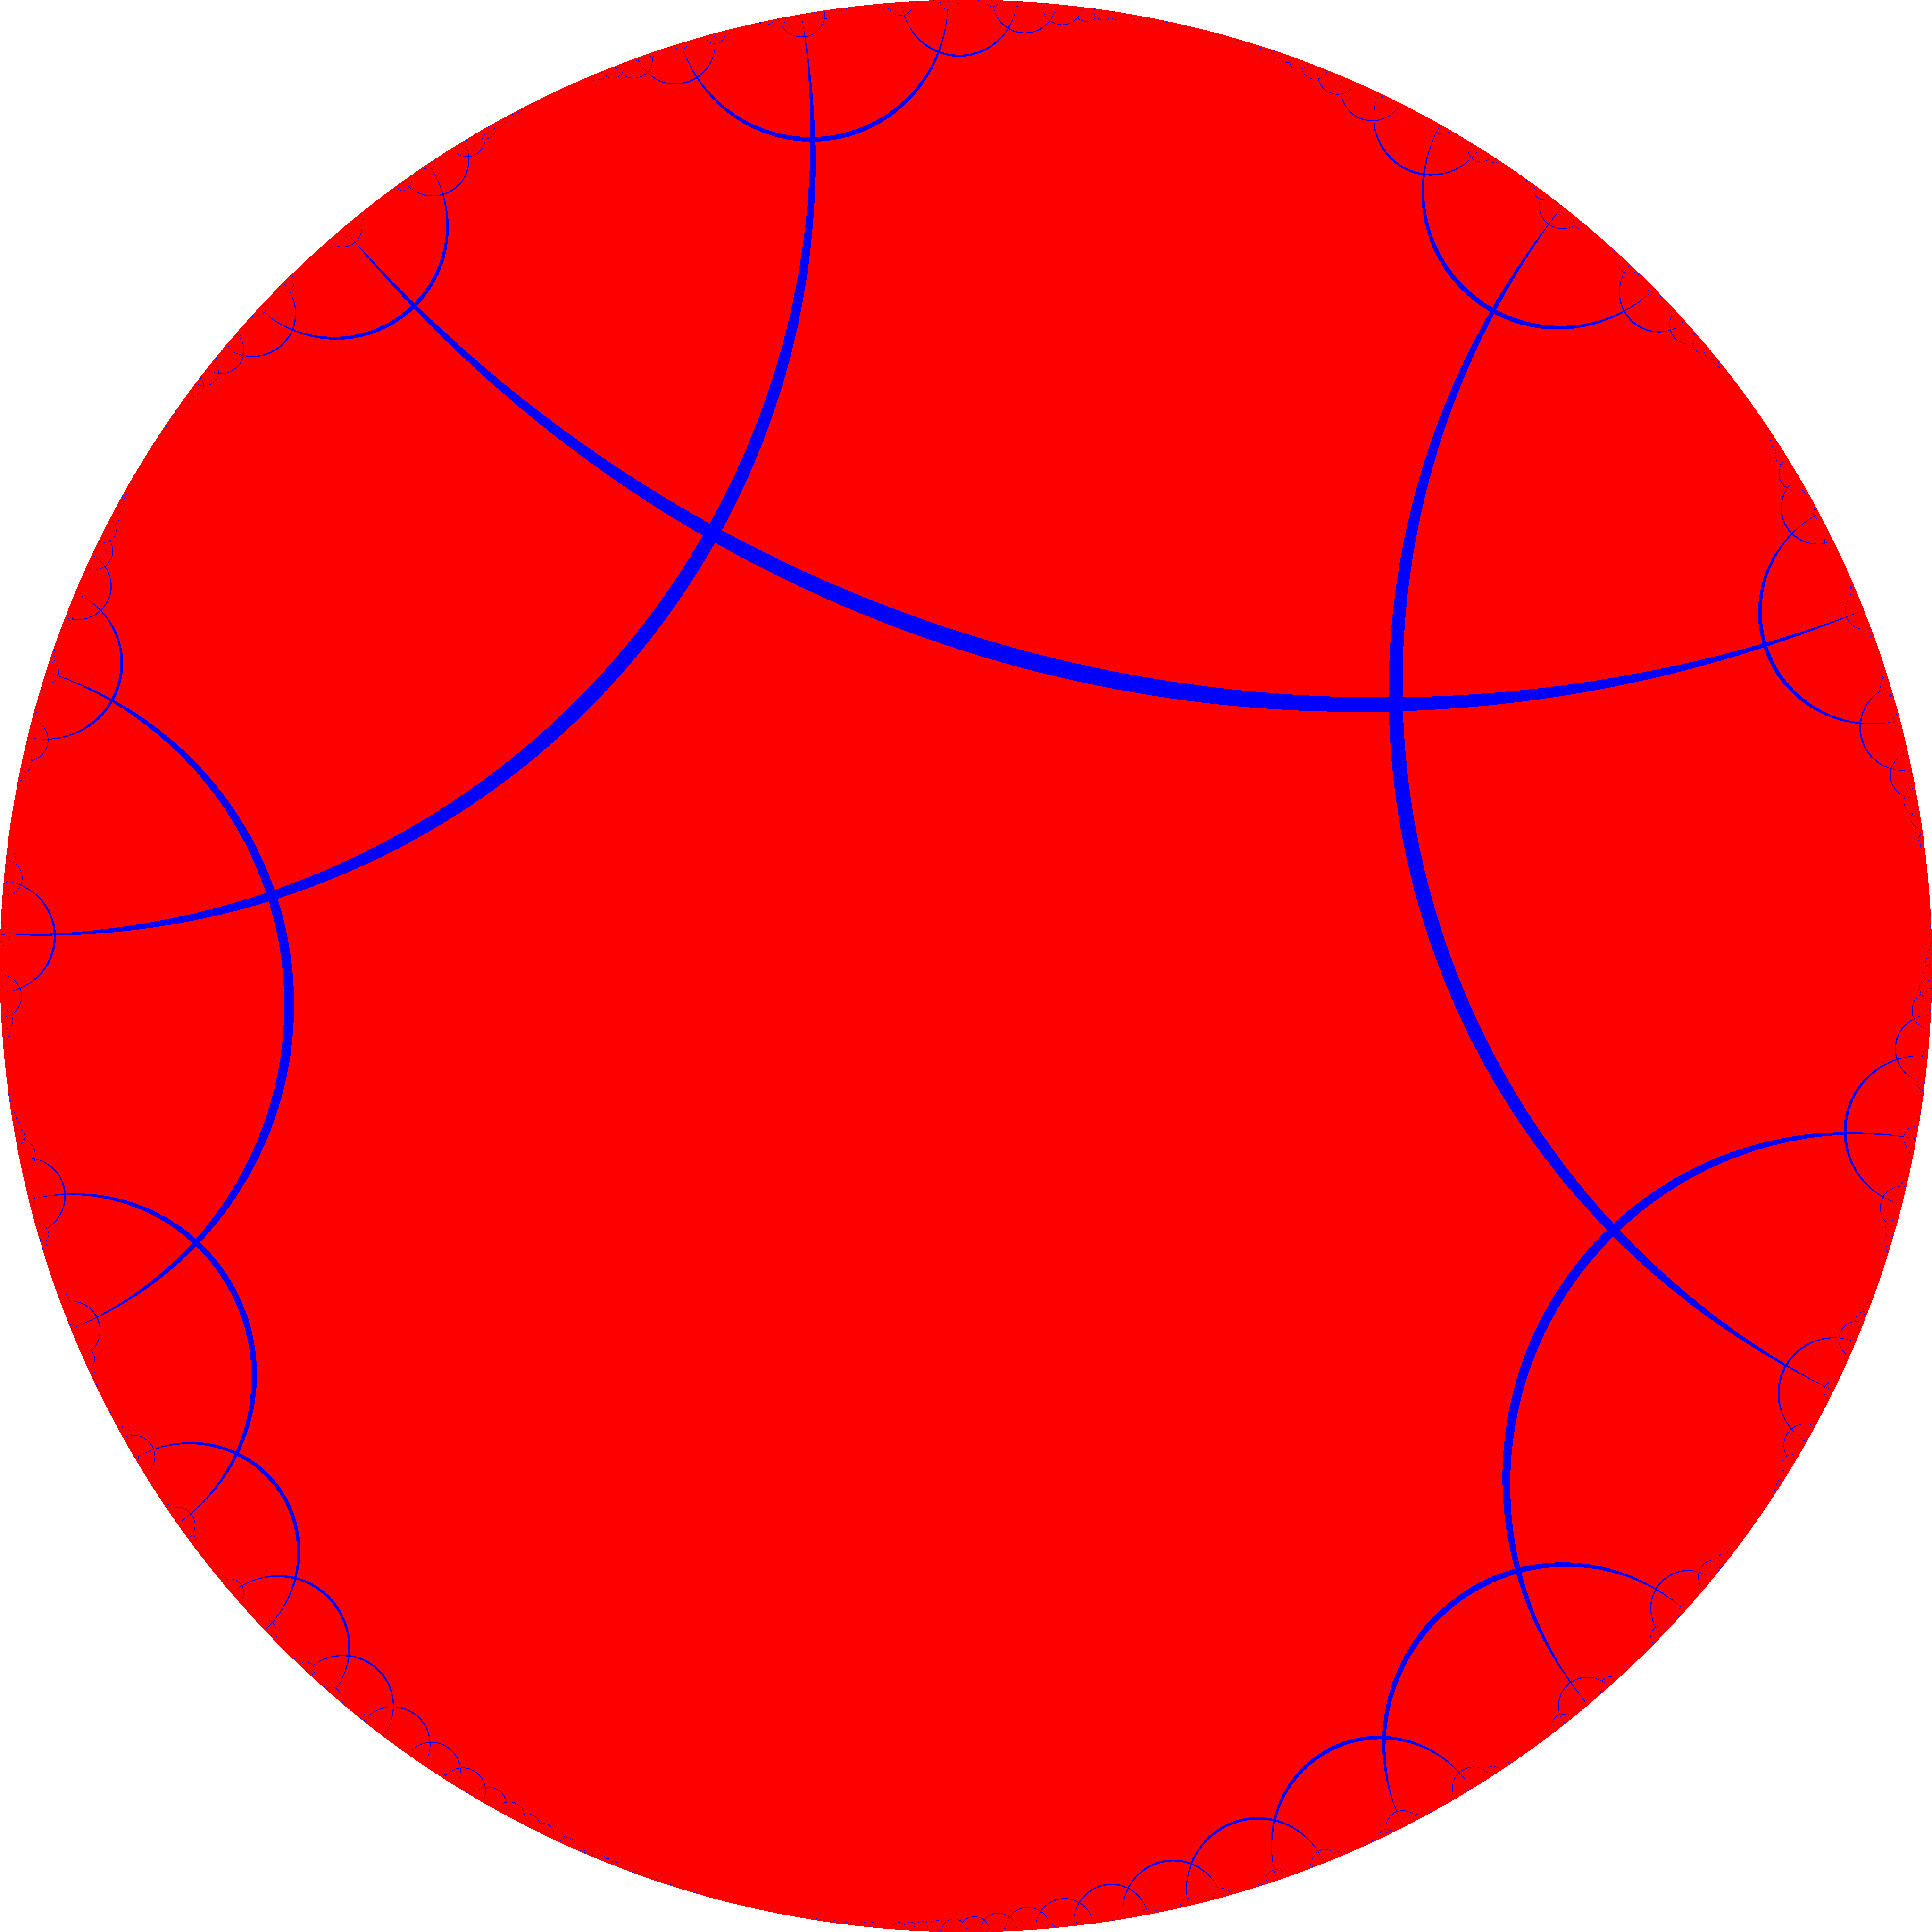
\includegraphics{images/t4096}}
\end{figure}
\end{frame}

\begin{frame}
\frametitle{The beginning point}
The famous example of word2vec
\begin{figure}[ht]
\centering
\resizebox{0.5\textwidth}{!}{
\begin{tikzpicture}[x=0.5cm,y=0.5cm,z=0.3cm,>=stealth]
\draw[->] (xyz cs:x=-7.0) -- (xyz cs:x=7.0) node[above] {$x_0$};
\draw[->] (xyz cs:y=0) -- (xyz cs:y=7.0) node[right] {$x_n$};
\draw[->] (xyz cs:z=-7.0) -- (xyz cs:z=7.0) node[above] {$x_i$};

\node[fill,circle,inner sep=1.5pt,label={left:$king$}] (p) at (xyz cs:x=-3.0, y=3.0, z=-3.0) {};
\node[fill,circle,inner sep=1.5pt,label={right:$man$}] (q) at (xyz cs:x=2.0, y=-3.0, z=3.0) {};
\node[fill,circle,inner sep=1.5pt,label={left:$queen$}] (r) at (xyz cs:x=-3.0, y=3.0, z=3.0) {};
\node[fill,circle,inner sep=1.5pt,label={right:$woman$}] (s) at (xyz cs:x=2.0, y=-3.0, z=9.0) {};
\draw[dashed, blue] (p) -- (q);
\draw[dashed, blue] (r) -- (s);
\draw[dashed, red] (p) -- (r);
\draw[dashed, red] (q) -- (s);
\end{tikzpicture}
}
\caption{regulairty of word2vec}
\label{fig:regulairty-of-word2vec}
\end{figure}
\end{frame}

\begin{frame}
\frametitle{The case of numbers}
\[
(\alpha + 1) \times 2 \neq \alpha \times 2 + 1
\]

\begin{figure}[ht]
\centering
\resizebox{0.5\textwidth}{!}{
\begin{tikzpicture}[x=0.5cm,y=0.5cm,z=0.3cm,>=stealth]
\draw[->] (xyz cs:x=-7.0) -- (xyz cs:x=7.0) node[above] {$x_0$};
\draw[->] (xyz cs:y=0) -- (xyz cs:y=7.0) node[right] {$x_n$};
\draw[->] (xyz cs:z=-7.0) -- (xyz cs:z=7.0) node[above] {$x_i$};

\node[fill,circle,inner sep=1.5pt,label={left:$\alpha$}] (p) at (xyz cs:x=-3.0, y=3.0, z=-3.0) {};
\node[fill,circle,inner sep=1.5pt,label={right:$\alpha+1$}] (q) at (xyz cs:x=2.0, y=-3.0, z=3.0) {};
\node[fill,circle,inner sep=1.5pt,label={left:$\alpha \times 2$}] (r) at (xyz cs:x=-3.0, y=3.0, z=3.0) {};
\node[fill,circle,inner sep=1.5pt,label={right:$(\alpha + 1) \times 2 \neq \alpha \times 2 + 1$}] (s) at (xyz cs:x=2.0, y=-3.0, z=9.0) {};
\draw[dashed, blue] (p) -- (q);
\draw[dashed, blue] (r) -- (s);
\draw[dashed, red] (p) -- (r);
\draw[dashed, red] (q) -- (s);
\end{tikzpicture}
}
\caption{contradicition of numbers in Euclidean space}
\label{fig:contradicition-of-numbers}
\end{figure}

\end{frame}

\begin{frame}
\frametitle{One arrangement in hyperbolic space}
\begin{figure}[ht]\centering
\resizebox{0.5\textwidth}{!}{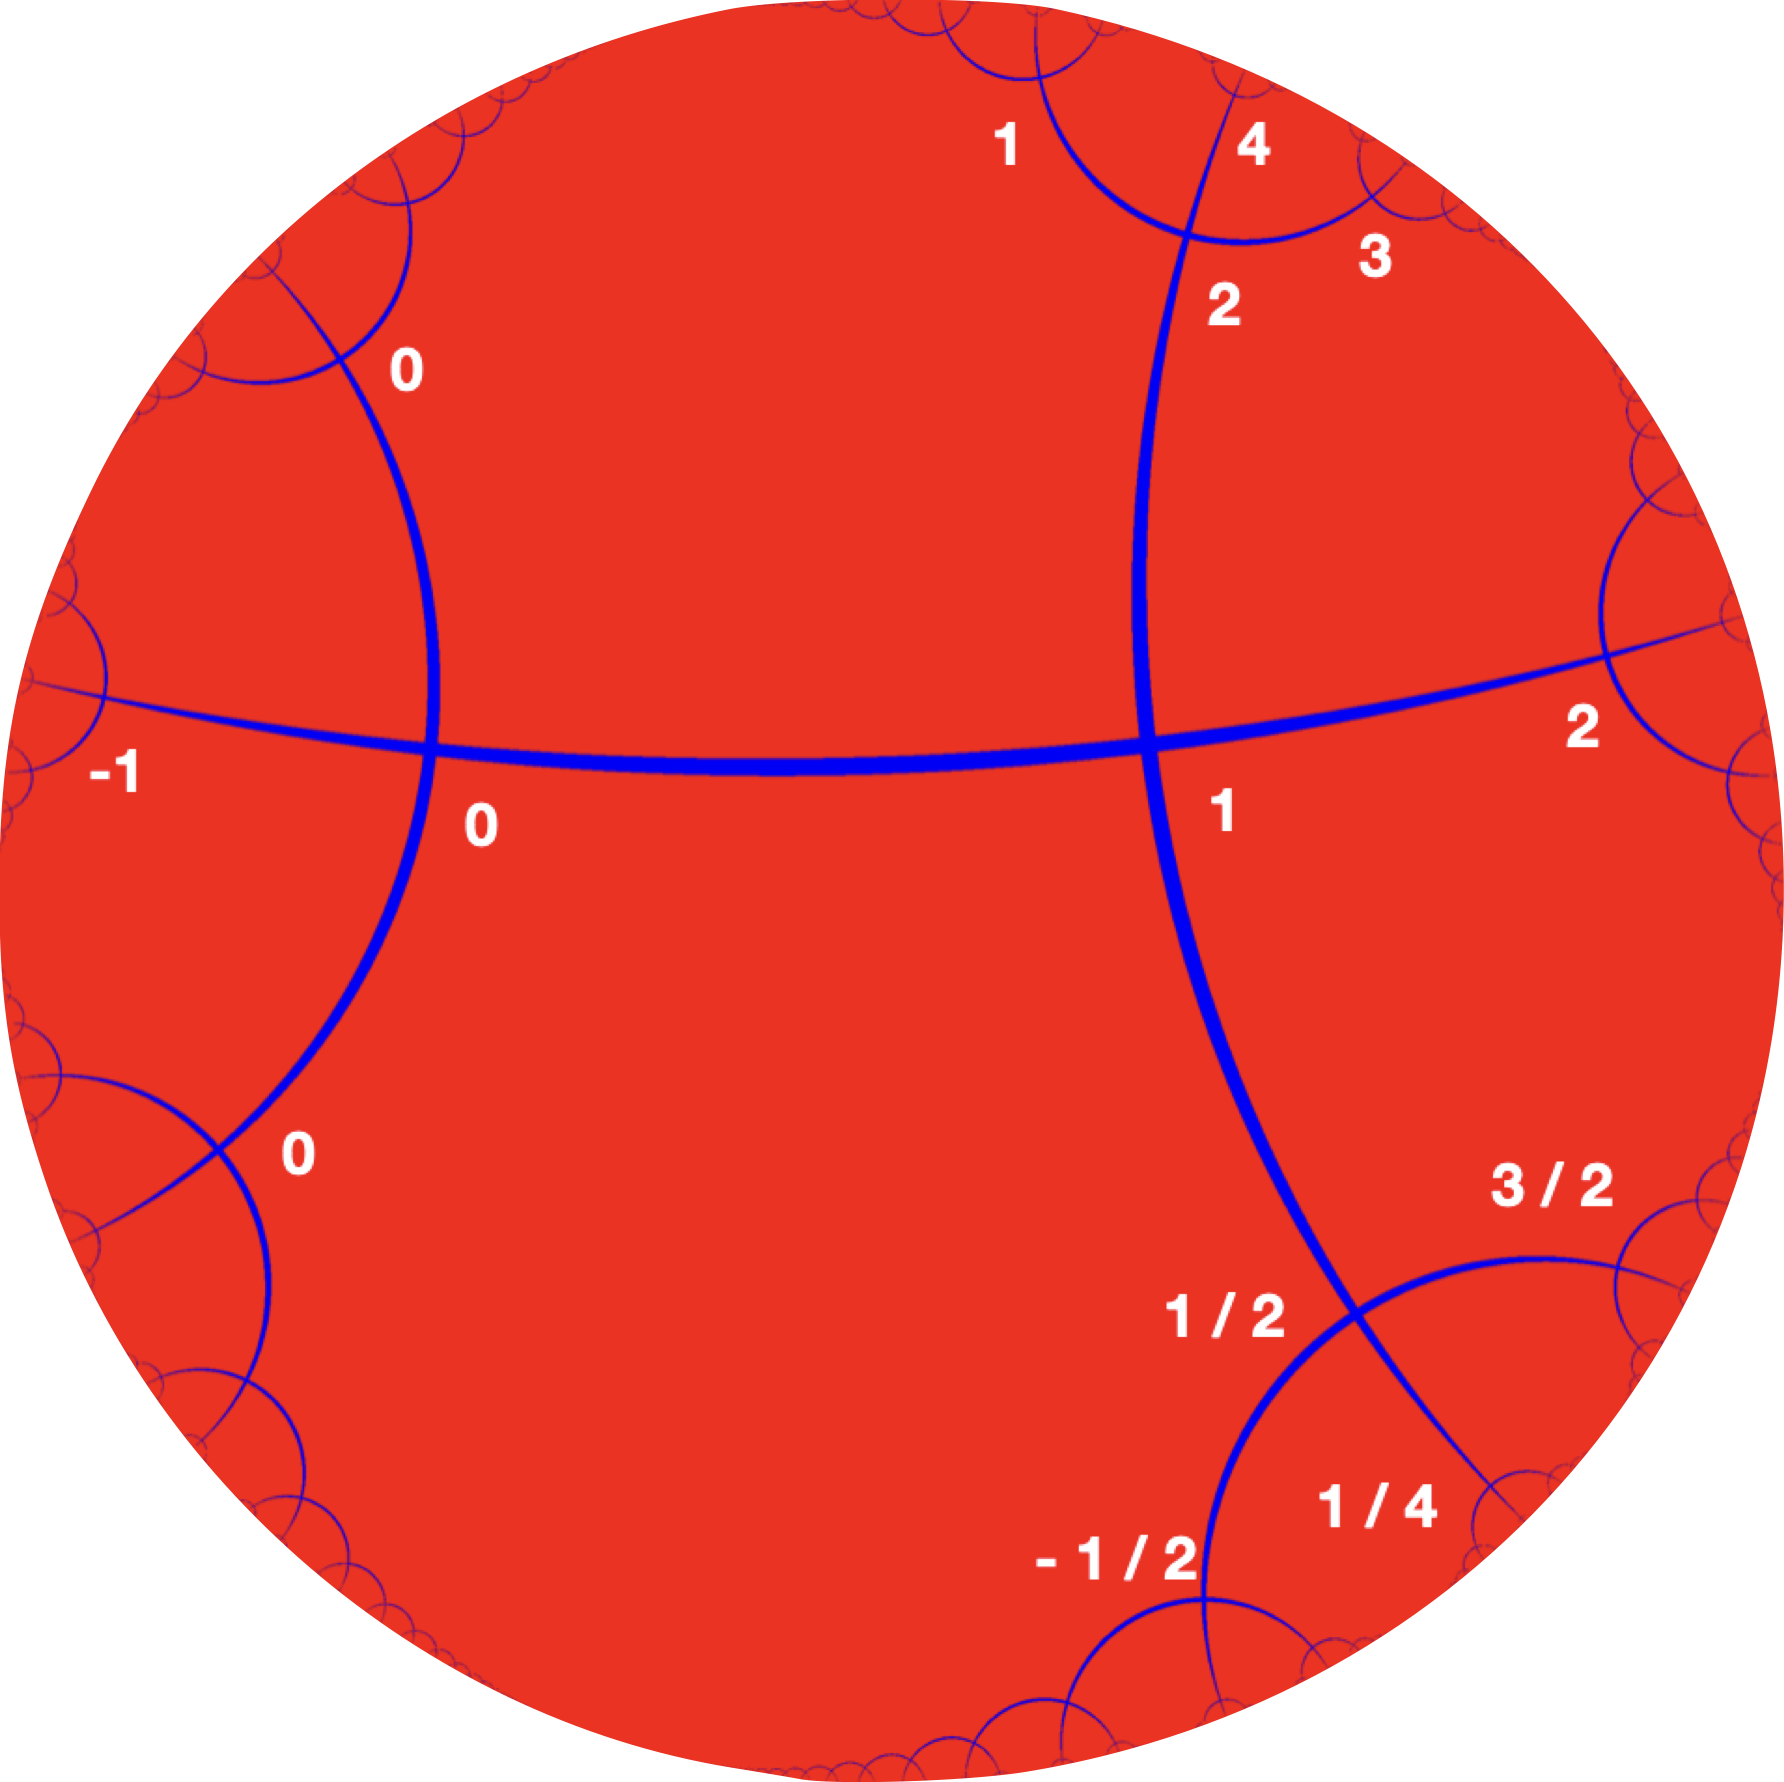
\includegraphics{images/assignment2}}
\end{figure}
\end{frame}

\begin{frame}
\frametitle{Another arrangement in hyperbolic space}
\begin{figure}[ht]
\centering
\resizebox{0.9\textwidth}{!}{
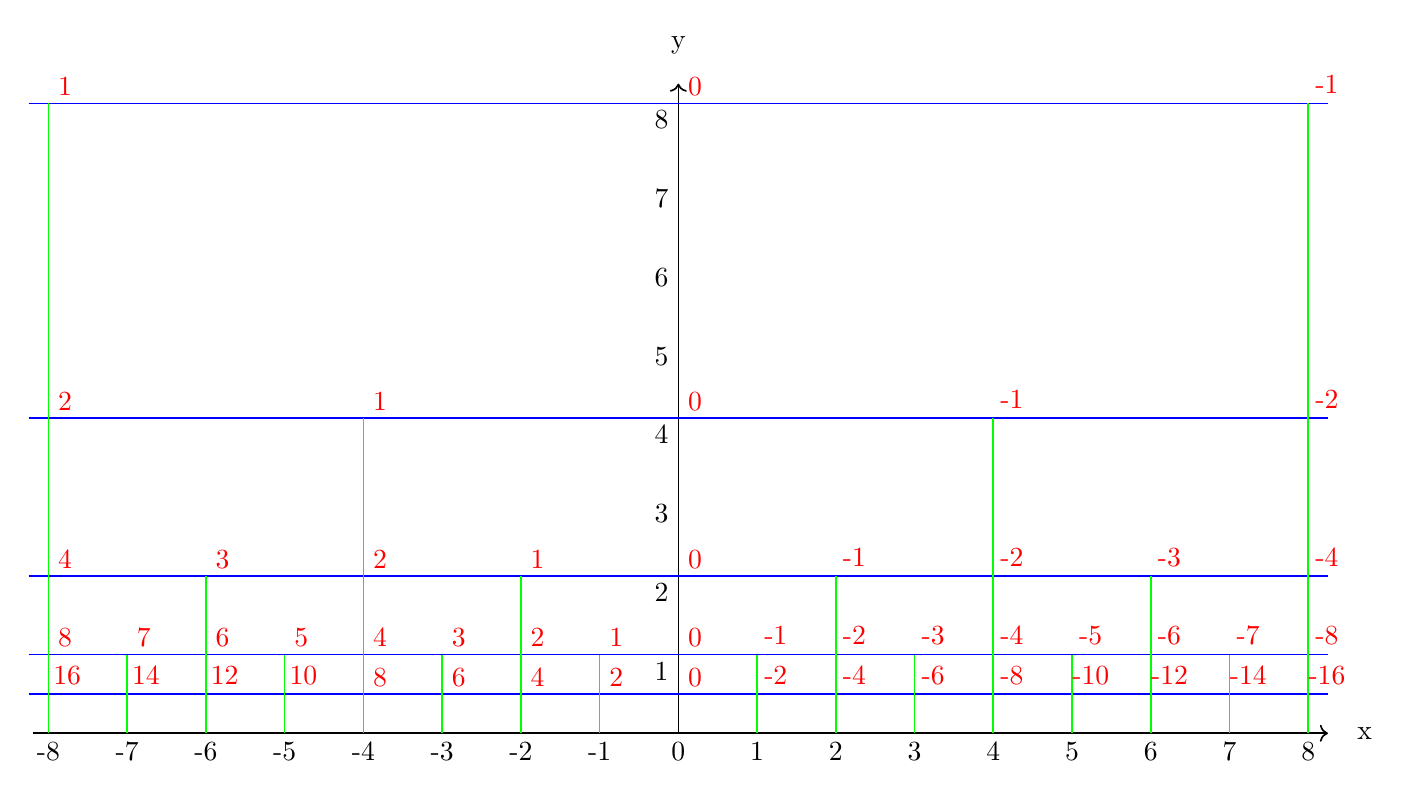
\begin{tikzpicture}
\draw [black, line width=0.6pt, ->] (0,0) to[out=90,in=270] (0,8.25);
\node [anchor=south] at (0,8.5) {y};
\draw [black, line width=0.6pt, ->] (-8.2,0) to[out=0,in=180] (8.25,0);
\node [anchor=west] at (8.5,0) {x};
\foreach \x in {-8,-7,-6,-5,-4,-3,-2,-1,0,1,2,3,4,5,6,7,8}
  \node [anchor=north] at (\x,0) {\x};
\foreach \y in {1,2,3,4,5,6,7,8}
  \node [anchor=45] at (0,\y) {\y};

\draw [blue, line width=0.6pt] (-8.25,0.5) to[out=0,in=180] (8.25,0.5);
\draw [blue, line width=0.6pt] (-8.25,1) to[out=0,in=180] (8.25,1);
\draw [blue, line width=0.6pt] (-8.25,2) to[out=0,in=180] (8.25,2);
\draw [blue, line width=0.6pt] (-8.25,4) to[out=0,in=180] (8.25,4);
\draw [blue, line width=0.6pt] (-8.25,8) to[out=0,in=180] (8.25,8);

\draw [green, line width=0.6pt] (-8,0) to[out=90,in=270] (-8,1);
\draw [green, line width=0.6pt] (-7,0) to[out=90,in=270] (-7,1);
\draw [green, line width=0.6pt] (-6,0) to[out=90,in=270] (-6,1);
\draw [green, line width=0.6pt] (-5,0) to[out=90,in=270] (-5,1);
\draw [green, line width=0.6pt] (-4,0) to[out=90,in=270] (-4,1);
\draw [green, line width=0.6pt] (-3,0) to[out=90,in=270] (-3,1);
\draw [green, line width=0.6pt] (-2,0) to[out=90,in=270] (-2,1);
\draw [green, line width=0.6pt] (-1,0) to[out=90,in=270] (-1,1);
\draw [green, line width=0.6pt] (1,0) to[out=90,in=270] (1,1);
\draw [green, line width=0.6pt] (2,0) to[out=90,in=270] (2,1);
\draw [green, line width=0.6pt] (3,0) to[out=90,in=270] (3,1);
\draw [green, line width=0.6pt] (4,0) to[out=90,in=270] (4,1);
\draw [green, line width=0.6pt] (5,0) to[out=90,in=270] (5,1);
\draw [green, line width=0.6pt] (6,0) to[out=90,in=270] (6,1);
\draw [green, line width=0.6pt] (7,0) to[out=90,in=270] (7,1);
\draw [green, line width=0.6pt] (8,0) to[out=90,in=270] (8,1);

\draw [green, line width=0.6pt] (-8,1) to[out=90,in=270] (-8,2);
\draw [green, line width=0.6pt] (-6,1) to[out=90,in=270] (-6,2);
\draw [green, line width=0.6pt] (-4,1) to[out=90,in=270] (-4,2);
\draw [green, line width=0.6pt] (-2,1) to[out=90,in=270] (-2,2);
\draw [green, line width=0.6pt] (2,1) to[out=90,in=270] (2,2);
\draw [green, line width=0.6pt] (4,1) to[out=90,in=270] (4,2);
\draw [green, line width=0.6pt] (6,1) to[out=90,in=270] (6,2);
\draw [green, line width=0.6pt] (8,1) to[out=90,in=270] (8,2);

\draw [green, line width=0.6pt] (-8,2) to[out=90,in=270] (-8,4);
\draw [green, line width=0.6pt] (-4,2) to[out=90,in=270] (-4,4);
\draw [green, line width=0.6pt] (4,2) to[out=90,in=270] (4,4);
\draw [green, line width=0.6pt] (8,2) to[out=90,in=270] (8,4);

\draw [green, line width=0.6pt] (-8,4) to[out=90,in=270] (-8,8);
\draw [green, line width=0.6pt] (8,4) to[out=90,in=270] (8,8);

\node [anchor=225, red] at (-8,0.5) {16};
\node [anchor=225, red] at (-7,0.5) {14};
\node [anchor=225, red] at (-6,0.5) {12};
\node [anchor=225, red] at (-5,0.5) {10};
\node [anchor=225, red] at (-4,0.5) {8};
\node [anchor=225, red] at (-3,0.5) {6};
\node [anchor=225, red] at (-2,0.5) {4};
\node [anchor=225, red] at (-1,0.5) {2};
\node [anchor=225, red] at (0,0.5) {0};
\node [anchor=225, red] at (1,0.5) {-2};
\node [anchor=225, red] at (2,0.5) {-4};
\node [anchor=225, red] at (3,0.5) {-6};
\node [anchor=225, red] at (4,0.5) {-8};
\node [anchor=225, red] at (5,0.5) {-10};
\node [anchor=225, red] at (6,0.5) {-12};
\node [anchor=225, red] at (7,0.5) {-14};
\node [anchor=225, red] at (8,0.5) {-16};

\node [anchor=225, red] at (-8,1) {8};
\node [anchor=225, red] at (-7,1) {7};
\node [anchor=225, red] at (-6,1) {6};
\node [anchor=225, red] at (-5,1) {5};
\node [anchor=225, red] at (-4,1) {4};
\node [anchor=225, red] at (-3,1) {3};
\node [anchor=225, red] at (-2,1) {2};
\node [anchor=225, red] at (-1,1) {1};
\node [anchor=225, red] at (0,1) {0};
\node [anchor=225, red] at (1,1) {-1};
\node [anchor=225, red] at (2,1) {-2};
\node [anchor=225, red] at (3,1) {-3};
\node [anchor=225, red] at (4,1) {-4};
\node [anchor=225, red] at (5,1) {-5};
\node [anchor=225, red] at (6,1) {-6};
\node [anchor=225, red] at (7,1) {-7};
\node [anchor=225, red] at (8,1) {-8};

\node [anchor=225, red] at (-8,2) {4};
\node [anchor=225, red] at (-6,2) {3};
\node [anchor=225, red] at (-4,2) {2};
\node [anchor=225, red] at (-2,2) {1};
\node [anchor=225, red] at (0,2) {0};
\node [anchor=225, red] at (2,2) {-1};
\node [anchor=225, red] at (4,2) {-2};
\node [anchor=225, red] at (6,2) {-3};
\node [anchor=225, red] at (8,2) {-4};

\node [anchor=225, red] at (-8,4) {2};
\node [anchor=225, red] at (-4,4) {1};
\node [anchor=225, red] at (0,4) {0};
\node [anchor=225, red] at (4,4) {-1};
\node [anchor=225, red] at (8,4) {-2};

\node [anchor=225, red] at (-8,8) {1};
\node [anchor=225, red] at (0,8) {0};
\node [anchor=225, red] at (8,8) {-1};

\end{tikzpicture}
}
\label{fig:gridex0}
\end{figure}
\end{frame}

\begin{frame}
\frametitle{Encoding threadlike expressions as paths}

\begin{itemize}
    \item black $1 \times 8 - 5 = 3$
    \item purple $(1 - \frac{5}{8}) \times 8 = 3$
    \item brown $(((1 - \frac{1}{8}) \times 2 - \frac{1}{2}) \times 2 - 1) \times 2 = 3$
    \item orange is a special integral
\end{itemize}

\begin{figure}[ht]
\centering
\resizebox{0.8\textwidth}{!}{
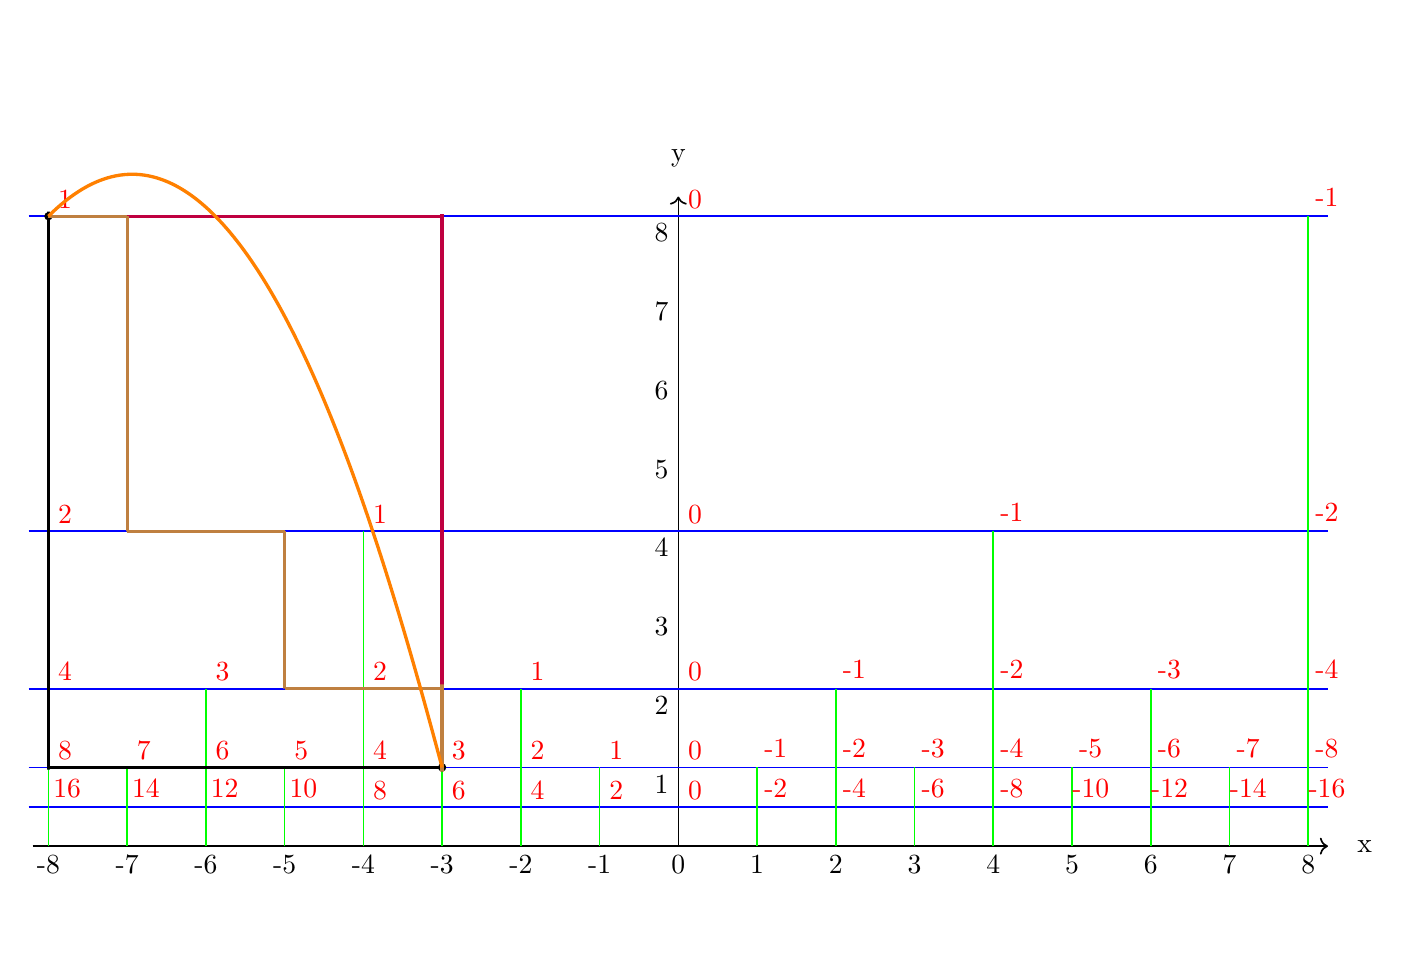
\begin{tikzpicture}
\draw [black, line width=0.6pt, ->] (0,0) to[out=90,in=270] (0,8.25);
\node [anchor=south] at (0,8.5) {y};
\draw [black, line width=0.6pt, ->] (-8.2,0) to[out=0,in=180] (8.25,0);
\node [anchor=west] at (8.5,0) {x};
\foreach \x in {-8,-7,-6,-5,-4,-3,-2,-1,0,1,2,3,4,5,6,7,8}
  \node [anchor=north] at (\x,0) {\x};
\foreach \y in {1,2,3,4,5,6,7,8}
  \node [anchor=45] at (0,\y) {\y};

\draw [blue, line width=0.6pt] (-8.25,0.5) to[out=0,in=180] (8.25,0.5);
\draw [blue, line width=0.6pt] (-8.25,1) to[out=0,in=180] (8.25,1);
\draw [blue, line width=0.6pt] (-8.25,2) to[out=0,in=180] (8.25,2);
\draw [blue, line width=0.6pt] (-8.25,4) to[out=0,in=180] (8.25,4);
\draw [blue, line width=0.6pt] (-8.25,8) to[out=0,in=180] (8.25,8);

\draw [green, line width=0.6pt] (-8,0) to[out=90,in=270] (-8,1);
\draw [green, line width=0.6pt] (-7,0) to[out=90,in=270] (-7,1);
\draw [green, line width=0.6pt] (-6,0) to[out=90,in=270] (-6,1);
\draw [green, line width=0.6pt] (-5,0) to[out=90,in=270] (-5,1);
\draw [green, line width=0.6pt] (-4,0) to[out=90,in=270] (-4,1);
\draw [green, line width=0.6pt] (-3,0) to[out=90,in=270] (-3,1);
\draw [green, line width=0.6pt] (-2,0) to[out=90,in=270] (-2,1);
\draw [green, line width=0.6pt] (-1,0) to[out=90,in=270] (-1,1);
\draw [green, line width=0.6pt] (1,0) to[out=90,in=270] (1,1);
\draw [green, line width=0.6pt] (2,0) to[out=90,in=270] (2,1);
\draw [green, line width=0.6pt] (3,0) to[out=90,in=270] (3,1);
\draw [green, line width=0.6pt] (4,0) to[out=90,in=270] (4,1);
\draw [green, line width=0.6pt] (5,0) to[out=90,in=270] (5,1);
\draw [green, line width=0.6pt] (6,0) to[out=90,in=270] (6,1);
\draw [green, line width=0.6pt] (7,0) to[out=90,in=270] (7,1);
\draw [green, line width=0.6pt] (8,0) to[out=90,in=270] (8,1);

\draw [green, line width=0.6pt] (-8,1) to[out=90,in=270] (-8,2);
\draw [green, line width=0.6pt] (-6,1) to[out=90,in=270] (-6,2);
\draw [green, line width=0.6pt] (-4,1) to[out=90,in=270] (-4,2);
\draw [green, line width=0.6pt] (-2,1) to[out=90,in=270] (-2,2);
\draw [green, line width=0.6pt] (2,1) to[out=90,in=270] (2,2);
\draw [green, line width=0.6pt] (4,1) to[out=90,in=270] (4,2);
\draw [green, line width=0.6pt] (6,1) to[out=90,in=270] (6,2);
\draw [green, line width=0.6pt] (8,1) to[out=90,in=270] (8,2);

\draw [green, line width=0.6pt] (-8,2) to[out=90,in=270] (-8,4);
\draw [green, line width=0.6pt] (-4,2) to[out=90,in=270] (-4,4);
\draw [green, line width=0.6pt] (4,2) to[out=90,in=270] (4,4);
\draw [green, line width=0.6pt] (8,2) to[out=90,in=270] (8,4);

\draw [green, line width=0.6pt] (-8,4) to[out=90,in=270] (-8,8);
\draw [green, line width=0.6pt] (8,4) to[out=90,in=270] (8,8);

\node [anchor=225, red] at (-8,0.5) {16};
\node [anchor=225, red] at (-7,0.5) {14};
\node [anchor=225, red] at (-6,0.5) {12};
\node [anchor=225, red] at (-5,0.5) {10};
\node [anchor=225, red] at (-4,0.5) {8};
\node [anchor=225, red] at (-3,0.5) {6};
\node [anchor=225, red] at (-2,0.5) {4};
\node [anchor=225, red] at (-1,0.5) {2};
\node [anchor=225, red] at (0,0.5) {0};
\node [anchor=225, red] at (1,0.5) {-2};
\node [anchor=225, red] at (2,0.5) {-4};
\node [anchor=225, red] at (3,0.5) {-6};
\node [anchor=225, red] at (4,0.5) {-8};
\node [anchor=225, red] at (5,0.5) {-10};
\node [anchor=225, red] at (6,0.5) {-12};
\node [anchor=225, red] at (7,0.5) {-14};
\node [anchor=225, red] at (8,0.5) {-16};

\node [anchor=225, red] at (-8,1) {8};
\node [anchor=225, red] at (-7,1) {7};
\node [anchor=225, red] at (-6,1) {6};
\node [anchor=225, red] at (-5,1) {5};
\node [anchor=225, red] at (-4,1) {4};
\node [anchor=225, red] at (-3,1) {3};
\node [anchor=225, red] at (-2,1) {2};
\node [anchor=225, red] at (-1,1) {1};
\node [anchor=225, red] at (0,1) {0};
\node [anchor=225, red] at (1,1) {-1};
\node [anchor=225, red] at (2,1) {-2};
\node [anchor=225, red] at (3,1) {-3};
\node [anchor=225, red] at (4,1) {-4};
\node [anchor=225, red] at (5,1) {-5};
\node [anchor=225, red] at (6,1) {-6};
\node [anchor=225, red] at (7,1) {-7};
\node [anchor=225, red] at (8,1) {-8};

\node [anchor=225, red] at (-8,2) {4};
\node [anchor=225, red] at (-6,2) {3};
\node [anchor=225, red] at (-4,2) {2};
\node [anchor=225, red] at (-2,2) {1};
\node [anchor=225, red] at (0,2) {0};
\node [anchor=225, red] at (2,2) {-1};
\node [anchor=225, red] at (4,2) {-2};
\node [anchor=225, red] at (6,2) {-3};
\node [anchor=225, red] at (8,2) {-4};

\node [anchor=225, red] at (-8,4) {2};
\node [anchor=225, red] at (-4,4) {1};
\node [anchor=225, red] at (0,4) {0};
\node [anchor=225, red] at (4,4) {-1};
\node [anchor=225, red] at (8,4) {-2};

\node [anchor=225, red] at (-8,8) {1};
\node [anchor=225, red] at (0,8) {0};
\node [anchor=225, red] at (8,8) {-1};

\node[circle,fill=black,inner sep=1pt,minimum size=3pt] (a) at (-8,8) {};
\node[circle,fill=black,inner sep=1pt,minimum size=3pt] (b) at (-3,1) {};

\draw [black, line width=1.2pt] (-8,7.7) to[out=90,in=270] (-8,1.33);
\draw [black, line width=1.2pt] (-8,1) to[out=0,in=180] (-3,1);

\draw [purple, line width=1.2pt] (-8,8) to[out=0,in=180] (-3,8);
\draw [purple, line width=1.2pt] (-3,7.67) to[out=90,in=270] (-3,1.33);

\draw [brown, line width=1.2pt] (-8,8) to[out=0,in=180] (-7,8);
\draw [brown, line width=1.2pt] (-7,7.8) to[out=90,in=270] (-7,4.2);
\draw [brown, line width=1.2pt] (-7,4) to[out=0,in=180] (-5,4);
\draw [brown, line width=1.2pt] (-5,3.9) to[out=90,in=270] (-5,2.1);
\draw [brown, line width=1.2pt] (-5,2) to[out=0,in=180] (-3,2);
\draw [brown, line width=1.2pt] (-3,2) to[out=90,in=270] (-3,1);

\draw [orange, line width=1.2pt] (-8,8) to[out=45,in=105] (-3,1);

\end{tikzpicture}
}
\label{fig:pathex1}
\end{figure}

\end{frame}

\begin{frame}
\frametitle{The flow equation}

\[
    a_{\delta} = (a_0 + \mu \epsilon \cos \theta)e^{\lambda \epsilon \sin \theta}
\]

\[
    a_{\delta} = a_0 e^{\lambda \epsilon \sin \theta} + \mu \epsilon \cos \theta
\]

\end{frame}

\begin{frame}
\frametitle{The flow equation}

Both formula can be simplified to the same result:

\[
    a_{\delta} = a_0 + \epsilon (a_0 \lambda \sin \theta + \mu \cos \theta)
\]

Then, we have the following equation:

\[
    \frac{1}{\delta} (a_{\delta} - a_0) = \frac{\epsilon}{\delta} (\mu \cos \theta + x_0 \lambda \sin \theta)
\]

When both $\delta$ and $\epsilon$ are towards zero, we get $da / dt$, and hence

\[
    \frac{da}{dt} = u (\mu \cos \theta + a \lambda \sin \theta)
\]

Or, we can change it to another form

\begin{equation}
    \frac{da}{ds} = \mu \cos \theta + a \lambda \sin \theta\label{eq:flow}
\end{equation}

\end{frame}


\section{The efficiency of gradient learning}

\begin{frame}
\frametitle{The efficiency of gradient learning}
\begin{itemize}
    \item The efficiency of gradient learning
\end{itemize}
\end{frame}

\section{A learnable non-linearity}

\begin{frame}
\frametitle{A learnable non-linearity}
\begin{itemize}
    \item The efficiency of gradient learning
\end{itemize}
\end{frame}

\section{Arithmetic expression geometry: more topics}

\begin{frame}
\frametitle{Arithmetic expression geometry: more topics}
\begin{itemize}
    \item The efficiency of gradient learning
\end{itemize}
\end{frame}

\section{Perspcetives, future work, and unsolved problems}

\begin{frame}
\frametitle{Perspcetives, future work, and unsolved problems}
\begin{itemize}
    \item The efficiency of gradient learning
\end{itemize}

\end{frame}

\end{document}
